\documentclass[11pt,a4paper]{article}

\usepackage[utf8]{inputenc}
\usepackage[T1]{fontenc}
\usepackage{amsmath,amsthm}
\usepackage{newpxtext,newpxmath}
\usepackage[activate={true,nocompatibility},kerning=true]{microtype}
\usepackage[a4paper,textwidth=15cm,top=2.6cm,bottom=2.6cm,headsep=0.8cm]{geometry}
\usepackage{graphicx}
\usepackage{booktabs}
\usepackage{enumitem}
\usepackage{xcolor}
\usepackage[font=small,labelfont=sc,labelsep=period]{caption}
\usepackage{titlesec}
\usepackage{fancyhdr}
\usepackage[authoryear,round]{natbib}
\usepackage[colorlinks,allcolors=linkblue]{hyperref}

\definecolor{linkblue}{RGB}{30,60,110}
\emergencystretch=2em
\setlist{nosep}
\renewcommand{\bibfont}{\small}
\setlength{\bibsep}{2pt}

% Headings: small caps for sections, italics for subsections
\titleformat{\section}{\normalfont\large\scshape}{\thesection}{1em}{}
\titleformat{\subsection}{\normalfont\itshape}{\thesubsection}{1em}{}
\titlespacing*{\section}{0pt}{3ex plus 1ex}{1.5ex}
\titlespacing*{\subsection}{0pt}{2.5ex plus 1ex}{1ex}

% Running head with the short title, page number on the right
\pagestyle{fancy}
\fancyhf{}
\fancyhead[L]{\small\scshape ML statistical arbitrage after trading costs}
\fancyhead[R]{\small\thepage}
\renewcommand{\headrulewidth}{0.4pt}

\newcommand{\dd}{\mathop{}\!\mathrm{d}}
\theoremstyle{definition}
\newtheorem{Def}{Definition}
\theoremstyle{remark}
\newtheorem{Remark}{Remark}

\begin{document}

\thispagestyle{empty}
\begin{flushleft}
  {\LARGE ML Statistical Arbitrage\\[0.3ex] after Trading Costs\par}
  \vspace{1.5ex}
  \rule{\textwidth}{0.4pt}\par
  \vspace{1ex}
  {\scshape Jan Dylan Mahlinger}\hfill October 2026\par
\end{flushleft}

\vspace{3ex}
\begin{quote}
\small
\citet{krauss2017deep} show that machine-learning models trained on lagged
returns of S\&P~500 stocks earn large daily returns in a long-short strategy,
even after flat transaction costs that are the same for every stock and day.
I rebuild the strategy in simplified form with
gradient-boosted trees on CRSP data from 1990 to 2025 and ask how much of the
return survives stock-specific trading costs estimated from daily high and low
prices. With spread estimates floored at one tick, the net return is negative
over the full sample and in every year since 2009, and most of the net loss
comes from the stocks with the largest spreads. A holding buffer cuts the turnover by a
fifth to a third at almost no loss of gross return and reduces the net losses
considerably, but the strategy remains unprofitable after costs.
\end{quote}
\vspace{2ex}


\section{Introduction}

\citet{krauss2017deep} train deep neural networks, gradient-boosted trees
and random forests to predict whether an S\&P~500 stock will beat the
cross-sectional median on the next day. Buying the ten stocks with the highest
predicted probability and selling the ten with the lowest earns about
0.45\,\% per day before costs between 1992 and 2015 for an ensemble of the
three models. The paper accounts for trading costs with a flat 5 basis points
per half-turn for every stock and day, after which the ensemble still earns
0.25\,\% per day.

The strategy rebalances most of its portfolio every day, and a strategy that
buys recent losers may well trade the most expensive stocks at the most
expensive moments. The question of this project is therefore:

\begin{quote}
\emph{How much of the return of a machine-learning reversal strategy on the
S\&P~500 survives realistic, stock-specific trading costs?}
\end{quote}

To answer it, I
(i) rebuild the baseline in simplified form with one model, gradient-boosted
trees, and compare it with a simple reversal rule without machine learning;
(ii) estimate stock-specific bid-ask spreads with the estimator of
\citet{corwin2012simple}, compute net returns and split them by the spread
of the traded stocks; and
(iii) test whether a simple holding buffer, which reduces turnover, can
recover part of the net return.

The project relates to \citet{avramov2023machine}, who find that
machine-learning return predictability concentrates in hard-to-arbitrage stocks
and weakens after trading costs, and to \citet{nagel2012evaporating}, who
interprets short-term reversal profits as compensation for providing liquidity.


\section{Data}

Daily stock data and the point-in-time S\&P~500 membership come from CRSP via
Wharton Research Data Services (WRDS).

Wharton Research Data Services (WRDS) was used in preparing this project: ``ML
Statistical Arbitrage after Trading Costs''. This service and the data available
thereon constitute valuable intellectual property and trade secrets of WRDS
and/or its third-party suppliers.

A stock belongs to the universe on day $t$ if it is an index member on that
day. As in \citet{krauss2017deep}, daily data are downloaded for every stock
that was a member at some point between 1990 and 2025, for all of its trading
days in that period, since the features need up to 240 days of history. This
also keeps the delisting returns, which CRSP books on the day after the last
trading day and which usually lie outside the membership period.

The panel covers 9{,}067 trading days from January 1990 to December 2025,
1{,}326 stocks and 4.5 million stock-days with index membership. The number of
index members per day lies between 498 and 508; it is slightly above 500 from
2014 on because a few firms have two share classes in the index. On membership
days, returns, highs, lows and closing prices are never missing. The one daily
return above 100\,\% (2008) is a genuine price jump, not a data error. The condition
high $\ge \max(\text{open}, \text{close})$ and low $\le \min(\text{open},
\text{close})$ is violated in 5 of 4.2 million rows. The coverage by year is in
\texttt{results/data\_coverage.csv}.

The universe is not restricted to ordinary common shares. The usual share-code
filter would remove actual index members, mostly real estate investment trusts
and foreign-incorporated firms, which make up about 11\,\% of the membership
days in recent years.


\section{Method}

\subsection{Features and labels}

Features and labels follow \citet{krauss2017deep}. Let $r^s_t$ be the daily
return of stock $s$ on day $t$ (including dividends). The features are the
returns over the last $m$ trading days,
\[
  R^s_{t,m} = \prod_{j=t-m+1}^{t} \bigl(1 + r^s_j\bigr) - 1,
  \qquad m \in \{1, \dots, 20\} \cup \{40, 60, \dots, 240\},
\]
which gives 31 features per stock and day, using returns up to and including
day $t$ only. With $U_t$ the universe of day $t$, the label is
\[
  y^s_t = \mathbf{1}\Bigl\{ r^s_{t+1} > \operatorname{median}\{ r^j_{t+1} : j \in U_t \} \Bigr\},
\]
i.e., it asks whether a stock beats the median on the next day. Because of
the strict inequality, stocks exactly at the median get $y = 0$. In the early
1990s many daily returns are exactly zero, as prices were quoted in eighths of
a dollar, so slightly fewer than half of the labels are one.

\subsection{Study periods}

As in the paper, the sample is split into periods of 1000 trading days, with
750 days for training and the following 250 days for trading. The periods are
shifted by 250 days, so the trading windows follow each other without overlap.
The features are computed from the returns inside each period. The first 240
days therefore only serve as look-back, and the model is trained on the
remaining 510 days (about 255{,}000 observations). The first trading window
starts in December 1992, as in the paper; the last one ends in December 2025
and is shorter (67 days).

\subsection{Signals}

For each period, a LightGBM classifier is fitted on the training days and
predicts $\hat p^s_t = \mathbb{P}(y^s_t = 1)$ for the trading days. The
settings follow the paper: 100 trees of depth 3, learning rate 0.1 and about
half of the features considered at each split. The paper also uses a random
forest, a deep neural network and an ensemble of all three. I deliberately restrict myself to one model. The focus of this project is on
trading costs, not on comparing forecasting methods, and one model with a
realistic gross return is enough to measure how much of that return survives
the costs. Testing the other models is left for later work.

The benchmark needs no model at all. It ranks the stocks by minus their return
on day $t$, i.e., it buys the day's losers and sells the day's winners.
Comparing the two signals shows how much the machine-learning model adds to
plain short-term reversal.

\subsection{Portfolio and timing}

On each trading day $t$, the stocks are ranked by the signal. The strategy buys
the top $k$ and sells the bottom $k$ short, with equal weights, for
$k \in \{10, 50\}$. The gross return is
\[
  r^{\text{LS}} = \frac{1}{k} \sum_{s \in \text{long}} r^s - \frac{1}{k} \sum_{s \in \text{short}} r^s .
\]
In the main specification, as in the paper, the signal uses the closing prices
of day $t$, the portfolio is formed at the same close, and it earns the return
of day $t+1$. This is optimistic, because the closing price that generates the
signal is also assumed to be the execution price. As a check, the portfolio is
also formed one day later and earns the return of day $t+2$. Ties in the signal
are broken at random, and a missing return of a held stock counts as zero.

I report mean daily returns with $t$-statistics and annualized Sharpe ratios
(without a risk-free rate, since the portfolio is self-financing). To check for
look-ahead errors, the whole pipeline is run a second time with all features
replaced by random noise; if the timing is correct, the returns of this run
must be close to zero.


\section{Trading costs}

\subsection{Spread estimates}

Bid-ask spreads are not observed in the daily data, so I estimate them with the
method of \citet{corwin2012simple}. The daily high is usually a trade at the ask
and the daily low a trade at the bid, so the observed log range is the range of
the efficient price plus a spread component $\alpha = \ln\frac{1+S/2}{1-S/2}$.
The range of the efficient price grows with the square root of time, while the
spread component does not: a two-day range still contains the spread only once.
CRSP defines the daily high and low as the highest and lowest trading price of
the regular trading day and leaves them empty on days without a
trade,\footnote{CRSP US Stock \& Indexes Database Guide, data items
\texttt{DlyHigh} and \texttt{DlyLow}.} so the estimator is always fed with
trade prices and never with quotes.

Let $H_t$ and $L_t$ be the high and low of day $t$, and let
$H_{t-1,t} = \max(H_{t-1}, H_t)$ and $L_{t-1,t} = \min(L_{t-1}, L_t)$ be the
high and low over the two days. The estimator combines the sum of the two
squared one-day log ranges and the squared two-day log range,
\[
  \beta_t = \Bigl[\ln\frac{H_{t-1}}{L_{t-1}}\Bigr]^2 + \Bigl[\ln\frac{H_t}{L_t}\Bigr]^2,
  \qquad
  \gamma_t = \Bigl[\ln\frac{H_{t-1,t}}{L_{t-1,t}}\Bigr]^2,
\]
into
\[
  \alpha = \frac{\sqrt{2\beta} - \sqrt{\beta}}{3 - 2\sqrt{2}} - \sqrt{\frac{\gamma}{3 - 2\sqrt{2}}},
  \qquad
  S = \frac{2\,(e^{\alpha} - 1)}{1 + e^{\alpha}} .
\]
Before computing the ranges, overnight price jumps are removed. If the low of
day $t$ is above the close of day $t-1$, the high and low of day $t$ are
lowered by the difference, and vice versa. Pairs of days with a stock split in
between are skipped.

A single two-day estimate is very noisy and often negative. Corwin and Schultz
discuss setting negative two-day estimates to zero before averaging. In my
simulations with a known spread, this overstates small spreads by a factor of
two to four, because it removes only the negative estimation errors. I
therefore average the two-day estimates over the last 21 trading days and
floor only the average. The estimate for day $t$ uses prices up to day $t$
only.

A quoted spread cannot be smaller than the minimum price increment. In the main
specification, the 21-day average is therefore floored at one tick relative to
the closing price: one eighth of a dollar until June 1997, one sixteenth until
January 2001 and one cent afterwards (the dates of the earlier of the NYSE and
Nasdaq switches). Without this floor, the estimate is zero for most stocks in
the early 1990s, although spreads were certainly larger then than today. As a
robustness check, the average is floored at zero instead.

With few trades per day, the observed high and low miss part of the true
range, so the spread is underestimated. In the simulation, the estimator
recovers about 80\,\% of the true spread with 390 trades per day and almost all
of it with 2{,}000, so the estimates for the early years are, if anything, too
low.

\subsection{Turnover and net returns}

The portfolio has weights $w_{i,t} = +1/k$ for the long stocks, $-1/k$ for the
short stocks and zero otherwise. The daily turnover is
$\mathrm{TO}_t = \sum_i |w_{i,t} - w_{i,t-1}|$. Replacing the whole portfolio
gives $\mathrm{TO}_t = 4$, which corresponds to the four half-turns per day
assumed in the paper. Each unit traded costs half the spread, so the costs are
\[
  C^{\text{CS}}_t = \sum_i \frac{\hat S_{i,t}}{2}\, |w_{i,t} - w_{i,t-1}|,
  \qquad
  C^{\text{flat}}_t = 0.0005 \cdot \mathrm{TO}_t ,
\]
where $\hat S_{i,t}$ is the spread estimate on the day of the trade (for the
one-day lag, the day after the signal). A missing estimate is replaced by the
median estimate of that day. The net return is the gross return minus the
costs.

\subsection{Spread quintiles}

To see where the gross return and the costs come from, the index members are
sorted each day into five groups by their estimated spread, with quintile~1
holding the 20\,\% of stocks with the smallest spreads. The sort uses the mean
of the two-day estimates over the past 252 trading days (at least 126), before
any floor. The 21-day estimate used for the costs is too noisy for a sort,
especially for the volatile stocks that the strategy trades, and the tick floor
would give many stocks the same value. For each held stock, the gross
contribution $w_{i,t}\, r_{i,t+1}$ and the costs
$\tfrac{1}{2}\hat S_{i,t} |w_{i,t} - w_{i,t-1}|$ are assigned to its quintile on
the signal day. Summed over the quintiles, they give the gross return and the
costs of the portfolio.

\subsection{Holding buffer}

The baseline sells a stock as soon as it leaves the top (or bottom) $k$, even if
it only drops from rank $k$ to rank $k+1$, and often buys it back a day later.
The holding buffer uses different thresholds for buying and selling. A stock
enters the long leg only from the top $k$, as before, but a held stock is sold
only when it leaves the top $2k$; the short leg works the same way. Free places
are filled with the highest-ranked stocks of the top $k$ that are not yet held,
so each leg always holds $k$ stocks with weight $1/k$. A held stock in ranks
$k+1$ to $2k$ keeps its place, so a stock that enters the top $k$ is not bought
if no place is free. With a buffer of $k$
instead of $2k$, the rule is identical to the baseline. I fixed the buffer size
of $2k$ in advance and did not tune it.


\section{Results}

\subsection{Baseline before trading costs}

Table~\ref{tab:baseline} summarizes the gross returns. Over the trading period
of the paper (December 1992 to October 2015), the gradient-boosted trees earn
0.38\,\% per day for $k = 10$, almost exactly the 0.37\,\% that
\citet{krauss2017deep} report for their gradient-boosted trees. The share of
held positions on the correct side of the median is 53.3\,\% (paper: about
54\,\%), and the overall classification accuracy is 51.0\,\%. Returns fall with
$k$, as the stocks further from the top and bottom of the ranking carry a
weaker signal.

\begin{table}[ht]
\centering
\caption{Gross performance of the long-short portfolios. Mean daily return in
percent, $t$-statistic and annualized Sharpe ratio (no risk-free rate). Lag 0:
portfolio formed at the close of the signal day; lag 1: one day later.}
\label{tab:baseline}
\begin{tabular}{llrrrrrr}
\toprule
& & \multicolumn{3}{c}{1992--2015 (paper period)} & \multicolumn{3}{c}{1992--2025 (full sample)} \\
\cmidrule(lr){3-5} \cmidrule(lr){6-8}
Signal & $k$, lag & Mean & $t$ & Sharpe & Mean & $t$ & Sharpe \\
\midrule
Gradient-boosted trees & 10, 0 & 0.38 & 14.8 & 3.09 & 0.28 & 13.6 & 2.37 \\
                       & 10, 1 & 0.19 & 7.6 & 1.59 & 0.14 & 6.8 & 1.18 \\
                       & 50, 0 & 0.21 & 14.3 & 3.00 & 0.16 & 13.4 & 2.34 \\
                       & 50, 1 & 0.13 & 8.4 & 1.75 & 0.09 & 7.7 & 1.34 \\
\midrule
Simple reversal        & 10, 0 & 0.13 & 4.0 & 0.84 & 0.09 & 3.6 & 0.63 \\
                       & 10, 1 & 0.08 & 2.7 & 0.56 & 0.05 & 2.1 & 0.36 \\
                       & 50, 0 & 0.11 & 6.3 & 1.31 & 0.09 & 6.2 & 1.09 \\
                       & 50, 1 & 0.12 & 6.9 & 1.43 & 0.08 & 5.9 & 1.03 \\
\bottomrule
\end{tabular}
\end{table}

\begin{figure}[ht]
\centering
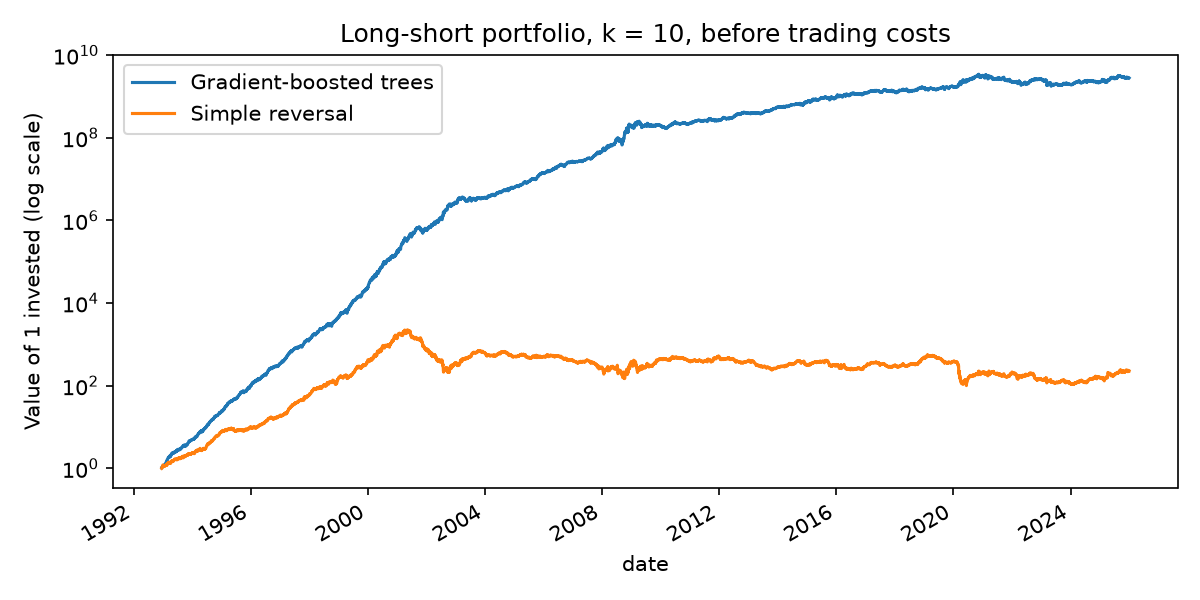
\includegraphics[width=0.85\textwidth]{../results/baseline/cumulative_returns.png}
\caption{Value of one unit invested in the long-short portfolio ($k = 10$,
lag 0) before trading costs, log scale.}
\label{fig:cumulative}
\end{figure}

Over the paper period, the gradient-boosted trees earn about three times as
much per day as the simple reversal rule (0.38\,\% versus 0.13\,\% for
$k = 10$). The simple rule stops working after 2001, while the model stays
clearly profitable until about 2008 (Figure~\ref{fig:cumulative}). Unlike the
simple rule, the model can also draw on the longer look-back returns.

Over time, the returns decline. For $k = 10$, the mean daily return of the
model is about 0.5--0.85\,\% in 1993--2002 and 0.1--0.3\,\% in 2003--2007. It is
high again in the financial crisis of 2008 (0.63\,\%) and mostly between 0
and 0.16\,\% from 2009 on, with 2020 as an exception (0.28\,\%) and negative
years in 2021 and 2023. This matches the decline reported in the paper and
continues after 2015.

A considerable part of the return depends on trading at the close that
produces the signal. With a one-day delay, the return of the model halves
(0.28\,\% to 0.14\,\% per day over the full sample) but stays significant. The
most likely reason is the bid-ask bounce. A stock whose closing trade happens
at the bid looks like a loser and seems to recover on the next day, although
an investor could not have bought it at that price.

In the leakage test, the hit rates are 50.0\,\% and seven of eight
specifications have $|t| < 1.3$; one has $t = 2.3$, which is within what one
expects by chance across eight tests. I find no sign of look-ahead.

\subsection{After trading costs}

Table~\ref{tab:costs} compares the gross returns with the net returns under
flat costs (5 bps per half-turn, as in the paper) and under the
Corwin-Schultz spread estimates. The model portfolio with $k = 10$ trades
2.74 units per day. This is about two thirds of the complete daily turnover of
4 that the paper assumes, since some stocks stay in the portfolio for several
days. The simple reversal rule trades more (3.72).

\begin{table}[ht]
\centering
\caption{Mean daily return in percent before and after costs (1992--2025),
average daily turnover, and break-even spread in basis points (the spread at
which the costs equal the gross return). Corwin-Schultz: spread estimate
floored at one tick (main specification) or at zero (robustness).}
\label{tab:costs}
\small
\begin{tabular}{llrrrrrr}
\toprule
& & & & \multicolumn{2}{c}{Corwin-Schultz} & & \\
\cmidrule(lr){5-6}
Signal & $k$, lag & Gross & Flat & Tick & Zero & Turnover & Break-even \\
\midrule
Gradient-boosted trees & 10, 0 & 0.279 & 0.142 & $-0.101$ & 0.018 & 2.74 & 20.4 \\
                       & 10, 1 & 0.138 & 0.001 & $-0.243$ & $-0.124$ & 2.74 & 10.1 \\
                       & 50, 0 & 0.162 & 0.048 & $-0.131$ & $-0.055$ & 2.29 & 14.2 \\
                       & 50, 1 & 0.093 & $-0.022$ & $-0.201$ & $-0.124$ & 2.29 & 8.1 \\
\midrule
Simple reversal        & 10, 0 & 0.093 & $-0.093$ & $-0.481$ & $-0.308$ & 3.72 & 5.0 \\
                       & 50, 0 & 0.092 & $-0.079$ & $-0.375$ & $-0.257$ & 3.41 & 5.4 \\
\bottomrule
\end{tabular}
\end{table}

With the flat costs of the paper, the model portfolio keeps about half of its
gross return over the full sample (0.14\,\% per day for $k = 10$). With a
one-day execution lag, nothing is left, and the simple reversal rule loses
money in every specification.

With the Corwin-Schultz estimates, every specification loses money after
costs. The model portfolio with $k = 10$ loses 0.10\,\% per day (Sharpe ratio
$-0.86$). On average it pays a spread of 28 bps per unit traded. That is more
than the median estimate of all index members (18 bps over the whole sample,
4--13 bps per year since 2010), because the strategy trades the stocks with
the largest recent price moves. Year by year, the net return is positive only
in 1997--2002, 2005--2006 and 2008, plus December 1992, the first month of
trading. In 1993--1996 the gross return is still 0.5--0.65\,\% per day, but
with prices quoted in eighths of a dollar the strategy pays spreads of
58--72 bps, which is more than it earns.\footnote{The tick size also shows up
in the labels. Until 1997 only about 47.5\,\% of the training labels are one,
from 2001 on almost exactly 50\,\%. With prices moving in eighths (later
sixteenths) of a dollar, many daily returns were exactly zero and often equal
to the median, which gives label zero under the strict inequality.} With the
zero floor, the net return of the model portfolio is close to zero (0.02\,\% per
day, Sharpe ratio 0.15), and the difference to the tick floor comes almost
entirely from the 1990s.

\subsection{Reliability of the spread estimates}

For S\&P~500 stocks the true spread is small relative to the daily volatility,
so a single two-day estimate is mostly noise; in every year about 40\,\% of them
are negative. Even after averaging over 21 days, the tick floor binds for
32--51\,\% of the stock-days since 2001 and for about 90\,\% in 1990--1996, so
the costs of the early years are essentially the tick size relative to the
price. The yearly medians move in the expected direction (high in 2000--2002,
2008--2009 and 2020, low in the late 2010s), but the level per stock is
uncertain, and for the volatile stocks that the strategy trades in the 2010s I
suspect the estimates are too high. I therefore put more weight on the
break-even analysis, which does not depend on the estimator.

\begin{figure}[ht]
\centering
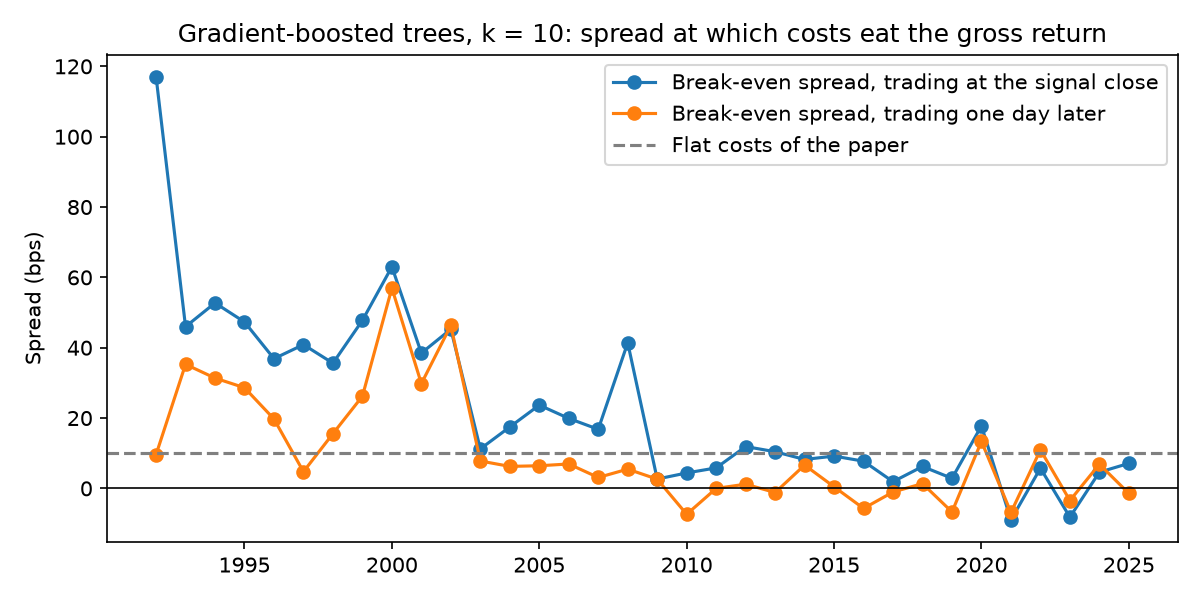
\includegraphics[width=0.85\textwidth]{../results/costs/breakeven_spread.png}
\caption{Break-even spread by year for the model portfolio ($k = 10$). The
dashed line marks the flat costs of the paper (5 bps per half-turn, i.e., a
spread of 10 bps).}
\label{fig:breakeven}
\end{figure}

Figure~\ref{fig:breakeven} shows, for each year, the spread at which the costs
would eat the whole gross return. Until 2002, the model portfolio could have
paid spreads of 36--63 bps and still made money. In 2003--2007 the break-even
spread falls to 11--24 bps, with a spike in 2008 (41 bps). From 2009 on it is
mostly between 2 and 12 bps, and in 2021 and 2023 it is negative. With a
one-day execution lag, it is close to zero from 2009 on. Quoted spreads of
large US stocks in the 2010s were in the range of a few basis points, and the
strategy trades the most volatile of them. I therefore conclude that the
strategy has not been profitable after costs since about 2009, with any of the
cost measures used here.

\subsection{Returns by spread quintile}

Table~\ref{tab:quintiles} splits the gross return and the costs of the model
portfolio by the spread quintile of the held stocks.

\begin{table}[ht]
\centering
\caption{Gradient-boosted trees, $k = 10$, lag 0 (1992--2025): share of held
positions, mean daily contribution to the gross return, the costs and the net
return in percent, and average spread paid per unit traded in basis points, by
spread quintile of the held stock (1 = smallest spreads).}
\label{tab:quintiles}
\begin{tabular}{lrrrrr}
\toprule
Quintile & Positions & Gross & Costs & Net & Spread paid \\
\midrule
1 (smallest spreads) & 0.32 & 0.073 & 0.077 & $-0.004$ & 18.4 \\
2                    & 0.18 & 0.039 & 0.050 & $-0.011$ & 20.2 \\
3                    & 0.15 & 0.047 & 0.049 & $-0.002$ & 23.5 \\
4                    & 0.15 & 0.036 & 0.057 & $-0.021$ & 28.0 \\
5 (largest spreads)  & 0.21 & 0.084 & 0.147 & $-0.063$ & 50.3 \\
\midrule
Total                & 1.00 & 0.279 & 0.380 & $-0.101$ & 27.7 \\
\bottomrule
\end{tabular}
\end{table}

\begin{figure}[ht]
\centering
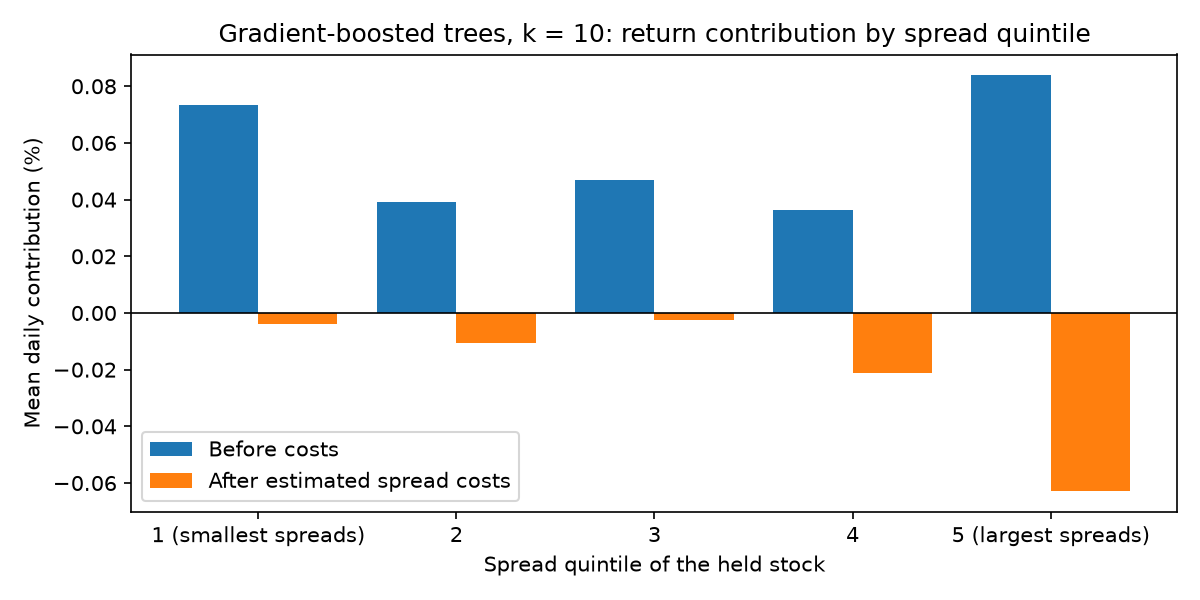
\includegraphics[width=0.85\textwidth]{../results/liquidity/returns_by_spread_quintile.png}
\caption{Mean daily contribution to the return of the model portfolio ($k = 10$,
lag 0) before and after the estimated spread costs, by spread quintile of the
held stock.}
\label{fig:quintiles}
\end{figure}

About a third of the positions fall into the quintile with the smallest spreads
and a fifth into the quintile with the largest, while the middle quintiles are
underrepresented. The strategy picks stocks with large recent price moves, and
the spread estimates of volatile stocks are noisier, which probably pushes them
into both outer quintiles. The sort still separates cheap from expensive
trades, with the spread paid rising from 18 bps in quintile~1 to 50 bps in
quintile~5.

Dividing the contribution of each quintile by its share of positions, a
position in quintile~5 earns about 0.40\,\% per day of portfolio return,
compared with 0.22--0.32\,\% in the other quintiles. The costs, however, grow
faster. Quintile~5 accounts for 39\,\% of the costs and for about 60\,\% of the
net loss (Figure~\ref{fig:quintiles}), whereas the most liquid quintile almost
breaks even.

For the simple reversal rule ($k = 10$, lag 0) the pattern is even stronger.
Quintile~5 delivers 0.072 of the 0.093\,\% gross return per day, and the most
liquid quintile contributes a negative gross return. This fits the view that
short-term reversal is a compensation for providing liquidity
\citep{nagel2012evaporating} and that it is largest where trading is most
expensive \citep{avramov2023machine}.

\subsection{Holding buffer}

Table~\ref{tab:buffer} compares the baseline with the holding buffer.

\begin{table}[ht]
\centering
\caption{Baseline (B) and holding buffer (H), 1992--2025. Columns as in
Table~\ref{tab:costs}; CS: Corwin-Schultz costs with tick floor.}
\label{tab:buffer}
\small
\setlength{\tabcolsep}{3pt}
\begin{tabular}{lllrrrrrr}
\toprule
Signal & $k$, lag & Rule & Turnover & Gross & Flat & CS & Sharpe CS & Break-even \\
\midrule
Gradient-boosted trees & 10, 0 & B & 2.74 & 0.279 & 0.142 & $-0.101$ & $-0.86$ & 20.4 \\
                       &       & H & 2.19 & 0.271 & 0.161 & $-0.032$ & $-0.27$ & 24.8 \\
                       & 10, 1 & B & 2.74 & 0.138 & 0.001 & $-0.243$ & $-2.08$ & 10.1 \\
                       &       & H & 2.19 & 0.136 & 0.027 & $-0.168$ & $-1.41$ & 12.4 \\
                       & 50, 0 & B & 2.29 & 0.162 & 0.048 & $-0.131$ & $-1.89$ & 14.2 \\
                       &       & H & 1.53 & 0.152 & 0.076 & $-0.046$ & $-0.66$ & 19.9 \\
                       & 50, 1 & B & 2.29 & 0.093 & $-0.022$ & $-0.201$ & $-2.89$ & 8.1 \\
                       &       & H & 1.53 & 0.082 & 0.005 & $-0.117$ & $-1.66$ & 10.7 \\
\midrule
Simple reversal        & 10, 0 & B & 3.72 & 0.093 & $-0.093$ & $-0.481$ & $-3.24$ & 5.0 \\
                       &       & H & 3.54 & 0.112 & $-0.066$ & $-0.436$ & $-2.92$ & 6.3 \\
                       & 50, 0 & B & 3.41 & 0.092 & $-0.079$ & $-0.375$ & $-4.37$ & 5.4 \\
                       &       & H & 3.01 & 0.103 & $-0.047$ & $-0.314$ & $-3.61$ & 6.9 \\
\bottomrule
\end{tabular}
\end{table}

\begin{figure}[ht]
\centering
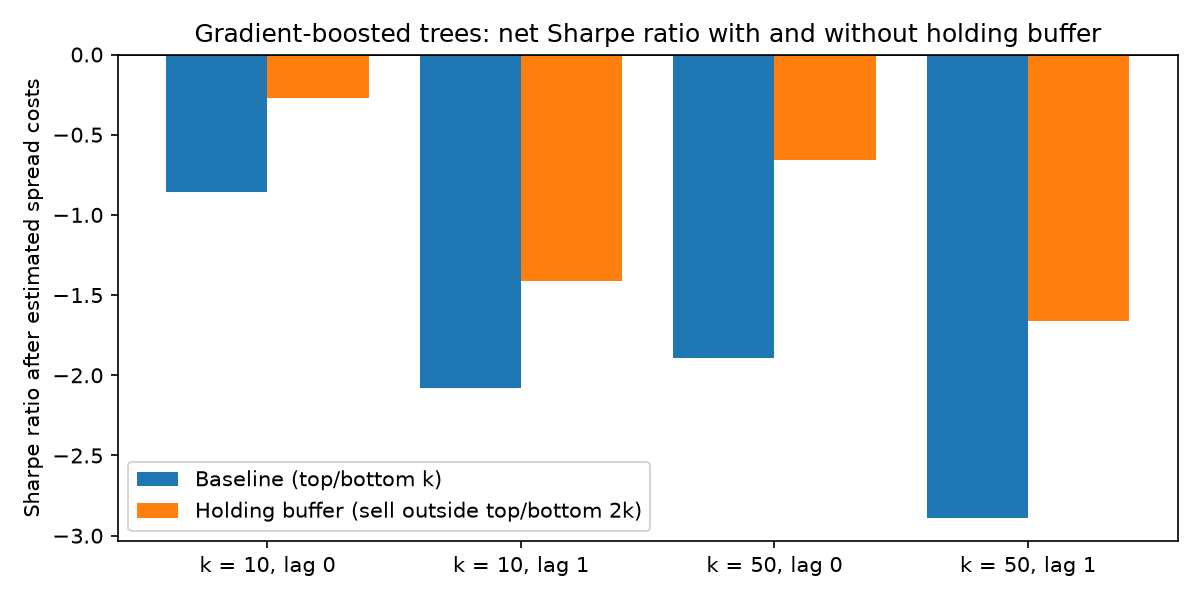
\includegraphics[width=0.85\textwidth]{../results/buffer/net_sharpe_buffer.png}
\caption{Sharpe ratio of the model portfolio after Corwin-Schultz costs, with
and without holding buffer.}
\label{fig:buffer}
\end{figure}

For the model portfolio, the buffer reduces the turnover by 20\,\% for
$k = 10$ and by 33\,\% for $k = 50$, while the gross return falls by only 3\,\%
and 6\,\%. The stocks that are kept although they dropped to ranks $k+1$ to
$2k$ still carry almost the same signal as the new candidates. For the simple
reversal rule, the turnover falls by only 5\,\% and 12\,\%, because a stock
among yesterday's biggest losers is rarely still among today's.

The break-even spread of the model portfolio with $k = 10$ rises from 20 to
25 bps, and the net loss after Corwin-Schultz costs shrinks from 0.10\,\% to
0.03\,\% per day (Figure~\ref{fig:buffer}). Year by year, the buffered portfolio is profitable after Corwin-Schultz costs in
1994, 1997--2002 and 2005--2008, but it still loses money in every year from
2009 on. In the recent period there is simply too little gross return left for
a lower turnover to make the strategy profitable.


\section{Limitations}

\begin{itemize}
  \item The baseline is a simplified rebuild of the paper with one model, not an
        exact replication. The random forest, the neural network and the
        ensemble of the paper are not tested yet.
  \item Execution at closing prices is optimistic; the one-day lag is only a
        partial check.
  \item Spreads are estimated from daily prices instead of being observed from
        quotes, and market impact is not modeled, so larger trades would pay more.
  \item Trades often happen inside the quotes, so the effective spread can be
        smaller than one tick, and the tick floor may overstate the costs of
        the 1990s. The zero floor gives the other extreme.
  \item Only one buffer size ($2k$) was tested.
\end{itemize}

\section*{Use of AI tools}

I designed and carried out this project myself: the research question, the
methodology, the choice of parameters, the robustness checks and the
interpretation of the results. I used the AI coding assistant Claude Code
(Anthropic) as a tool to speed up the implementation and to help edit this
text. All code was reviewed, tested and run by me. In line with the WRDS terms
of use, the assistant never had access to CRSP data.

\bibliographystyle{plainnat}
\bibliography{references}

\end{document}
